\documentclass[11pt,a4paper]{article}

\usepackage[margin=1.65cm,top=1.45cm,bottom=1.55cm]{geometry}
\usepackage{fontspec}
\usepackage{xeCJK}
\usepackage{booktabs}
\usepackage{tabularx}
\usepackage{array}
\usepackage{amsmath}
\usepackage{graphicx}
\usepackage{enumitem}
\usepackage[table]{xcolor}
\usepackage{microtype}
\usepackage{fancyhdr}
\usepackage[hidelinks]{hyperref}

\setCJKmainfont{Songti TC}
\setCJKsansfont{Heiti TC}
\IfFontExistsTF{TeX Gyre Pagella}{\setmainfont{TeX Gyre Pagella}}{}
\xeCJKsetup{CJKecglue=\hskip 0.10em plus 0.04em minus 0.04em}

\definecolor{accent}{HTML}{315A7D}
\definecolor{darkaccent}{HTML}{173B52}
\definecolor{lightrow}{HTML}{EEF3F7}
\definecolor{note}{HTML}{FFF4D8}
\setlength{\parindent}{0pt}
\setlength{\parskip}{0.38em}
\setlist[itemize]{leftmargin=1.45em,itemsep=0.12em,topsep=0.15em}
\renewcommand{\arraystretch}{1.16}
\newcolumntype{Y}{>{\raggedright\arraybackslash}X}
\newcolumntype{C}[1]{>{\centering\arraybackslash}p{#1}}
\graphicspath{{../figures/}}

\pagestyle{fancy}
\fancyhf{}
\fancyfoot[C]{\small\thepage}
\renewcommand{\headrulewidth}{0pt}
\newcommand{\q}[2]{\par\vspace{0.15em}\textcolor{accent}{\textbf{題 #1}}\hspace{0.8em}#2\par\nopagebreak[4]}
\newcommand{\metric}[1]{\texttt{#1}}
\newcommand{\compacttable}{\small\rowcolors{2}{lightrow}{white}}

\begin{document}
\hypersetup{pdftitle={HW5 分類器效能比較與模型選擇}}

\begin{center}
  {\LARGE\bfseries\color{darkaccent} HW5 分類器效能比較與模型選擇}\par
  \vspace{0.25em}
  {\small Part 2--5｜固定分層切分、Macro-F1 與 training-only 模型選擇}
\end{center}
\vspace{-0.6em}

\section*{Part 2：Dataset A 原始特徵 Baseline}
\vspace{-0.5em}

\q{4}{資料摘要與尺度。}
Breast Cancer Wisconsin 共有 569 筆、30 個連續特徵；類別為 malignant 212 筆、benign 357 筆。固定分層 80/20 切分後，訓練集 455 筆、測試集 114 筆。從下表的代表性特徵可以看出，數值尺度差距相當大：面積類特徵跨越數千，平滑度與 fractal dimension 僅約 $10^{-2}$ 至 $10^{-1}$。

\begin{center}
\compacttable
\begin{tabular*}{0.92\linewidth}{@{\extracolsep{\fill}}lrrrlrrr}
\toprule
特徵 & Min & Max & Range & 特徵 & Min & Max & Range \\
\midrule
mean radius & 6.981 & 28.110 & 21.129 & mean area & 143.5 & 2501.0 & 2357.5 \\
mean perimeter & 43.79 & 188.50 & 144.71 & area error & 6.802 & 542.200 & 535.398 \\
mean smoothness & 0.0526 & 0.1634 & 0.1108 & worst area & 185.2 & 4254.0 & 4068.8 \\
fractal dim. error & 0.0009 & 0.0298 & 0.0289 & worst concavity & 0.000 & 1.252 & 1.252 \\
\bottomrule
\end{tabular*}
\end{center}

\q{5}{事前假設。}
我預期 Random Forest 會在五個分類器中表現最好，因為多棵決策樹的集成能描述非線性特徵互動，同時以平均降低單棵樹的變異。SVM 可能也有競爭力，但本題 baseline 使用未標準化的原始特徵，RBF kernel 的距離幾何可能被數值尺度較大的特徵主導，因此不一定能在 baseline 階段領先。


\q{6}{未標準化的固定 baseline。}
五個模型共用相同的 455 筆訓練資料與 114 筆測試資料，並直接使用原始特徵。下表整理各模型的 Accuracy 與 Macro-F1。

\begin{center}
\compacttable
\begin{tabular*}{0.82\linewidth}{@{\extracolsep{\fill}}clllrr}
\toprule
排名 & 分類器 & 主要設定 & 前處理 & Accuracy & Macro-F1 \\
\midrule
1 & Random Forest & 200 trees, seed 42 & Raw & 0.9561 & 0.9526 \\
2 & Gaussian NB & defaults & Raw & 0.9386 & 0.9337 \\
3 & SVM & RBF, $C=1$ & Raw & 0.9298 & 0.9230 \\
4 & Decision Tree & seed 42 & Raw & 0.9123 & 0.9075 \\
5 & kNN & $k=5$ & Raw & 0.9123 & 0.9066 \\
\bottomrule
\end{tabular*}
\end{center}

\q{7}{排名與假設對照。}
以 Macro-F1 為主要排名依據、Accuracy 為次要依據，Random Forest 排名第一，與事前預期一致。SVM 排名第三，也符合原始特徵尺度可能影響 RBF kernel 的推測。Decision Tree 與 kNN 的 Accuracy 都是 0.9123，但 Decision Tree 的 Macro-F1 稍高。

\q{8}{不能宣稱第一名即全域最佳。}
這次只有一組訓練與測試資料切分，還無法判斷排名會不會隨抽樣而變動；各模型也尚未經過完整的超參數比較或前處理調整。此外，解釋性與運算成本同樣會影響實際選擇。因此，Random Forest 只能算是本次原始特徵 baseline 中表現最好的模型。

\section*{Part 3：Standardization 的影響}
\vspace{-0.5em}

\q{9}{無資料洩漏的標準化。}
\metric{StandardScaler} 只使用 455 筆訓練資料估計平均值與標準差，再以同一組參數轉換測試資料。資料切分及模型設定都維持不變，讓比較集中在標準化的影響。

\begin{minipage}{\linewidth}
\q{10}{四模型 Raw/Scaled 比較。}
\begin{center}
\compacttable
\begin{tabular}{lrrrrrr}
\toprule
分類器 & Raw Acc. & Scaled Acc. & $\Delta$Acc. & Raw F1 & Scaled F1 & $\Delta$F1 \\
\midrule
kNN & 0.9123 & 0.9561 & +0.0439 & 0.9066 & 0.9526 & +0.0460 \\
SVM & 0.9298 & 0.9825 & +0.0526 & 0.9230 & 0.9812 & +0.0582 \\
Decision Tree & 0.9123 & 0.9123 & 0.0000 & 0.9075 & 0.9075 & 0.0000 \\
Random Forest & 0.9561 & 0.9561 & 0.0000 & 0.9526 & 0.9526 & 0.0000 \\
\bottomrule
\end{tabular}
\end{center}
\end{minipage}

\q{11}{視覺比較。}
\begin{figure}[ht]
\centering
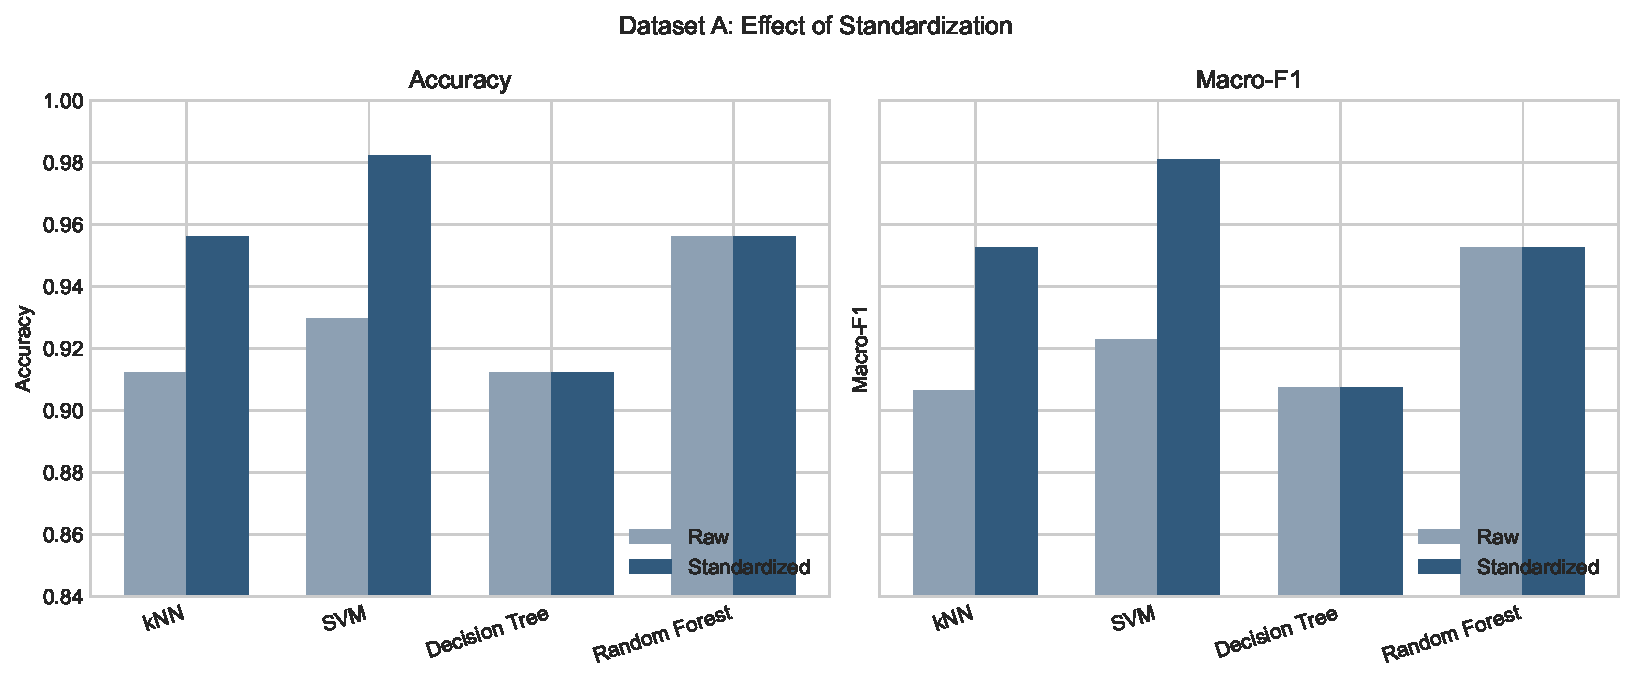
\includegraphics[width=0.78\linewidth]{standardization_comparison.pdf}
\caption{Dataset A 的 Raw/Scaled Accuracy 與 Macro-F1；圖值直接讀自 \metric{scaling\_a.csv}。}
\end{figure}

\q{12}{變化機制。}
SVM 的 Macro-F1 增加最多（+0.0582），其次是 kNN（+0.0460）。兩者都會受到特徵距離影響，若直接使用原始數值，area 等數值範圍大的特徵容易主導計算。標準化後，各特徵的影響較為均衡。相較之下，決策樹主要依單一特徵的大小順序決定分割點，因此這次 Decision Tree 與 Random Forest 的分數都沒有變化。

\q{13}{是否一定提升？}
不一定。這次 kNN 與 SVM 在標準化後都有明顯進步，但 Decision Tree 和 Random Forest 的 Accuracy、Macro-F1 都沒有改變。是否需要標準化，仍應依模型的運作方式與實際結果判斷。

\section*{Part 4：Stratified CV 與 Hyperparameter Selection}
\vspace{-0.5em}

\q{14}{搜尋設計。}
只使用 Dataset A 的訓練資料，透過 \metric{StratifiedKFold(5, shuffle=True, random\_state=42)} 比較 13 組超參數設定，評估指標為 \metric{f1\_macro}。kNN 與 SVM 使用 Pipeline，確保每一折的 StandardScaler 都只從該折訓練資料學習；Decision Tree 使用原始特徵。測試集不參與參數選擇。

\q{15}{各候選五折平均與母體標準差（\texttt{ddof=0}）。}
\begin{center}
\scriptsize
\rowcolors{2}{lightrow}{white}
\begin{tabular}{llrr@{\qquad}llrr@{\qquad}llrr}
\toprule
模型 & 設定 & Mean & Std & 模型 & 設定 & Mean & Std & 模型 & 設定 & Mean & Std \\
\midrule
kNN & $k=1$ & .9434 & .0201 & Tree & $d=2$ & .9275 & .0202 & SVM & $C=.1$ & .9377 & .0180 \\
kNN & $k=3$ & .9596 & .0096 & Tree & $d=3$ & .9204 & .0091 & SVM & $C=1$ & .9669 & .0160 \\
kNN & $k=5$ & .9598 & .0118 & Tree & $d=5$ & .9188 & .0123 & SVM & $C=10$ & .9671 & .0136 \\
kNN & $k=9$ & .9620 & .0158 & Tree & $d=10$ & .9119 & .0190 & & & & \\
kNN & $k=15$ & .9570 & .0180 & Tree & $d=$None & .9119 & .0190 & & & & \\
\bottomrule
\end{tabular}
\end{center}
每一列另保留五個 fold 原始分數於 \metric{cv\_search\_a.csv}。

\begin{center}
\begin{minipage}{0.90\linewidth}
\centering
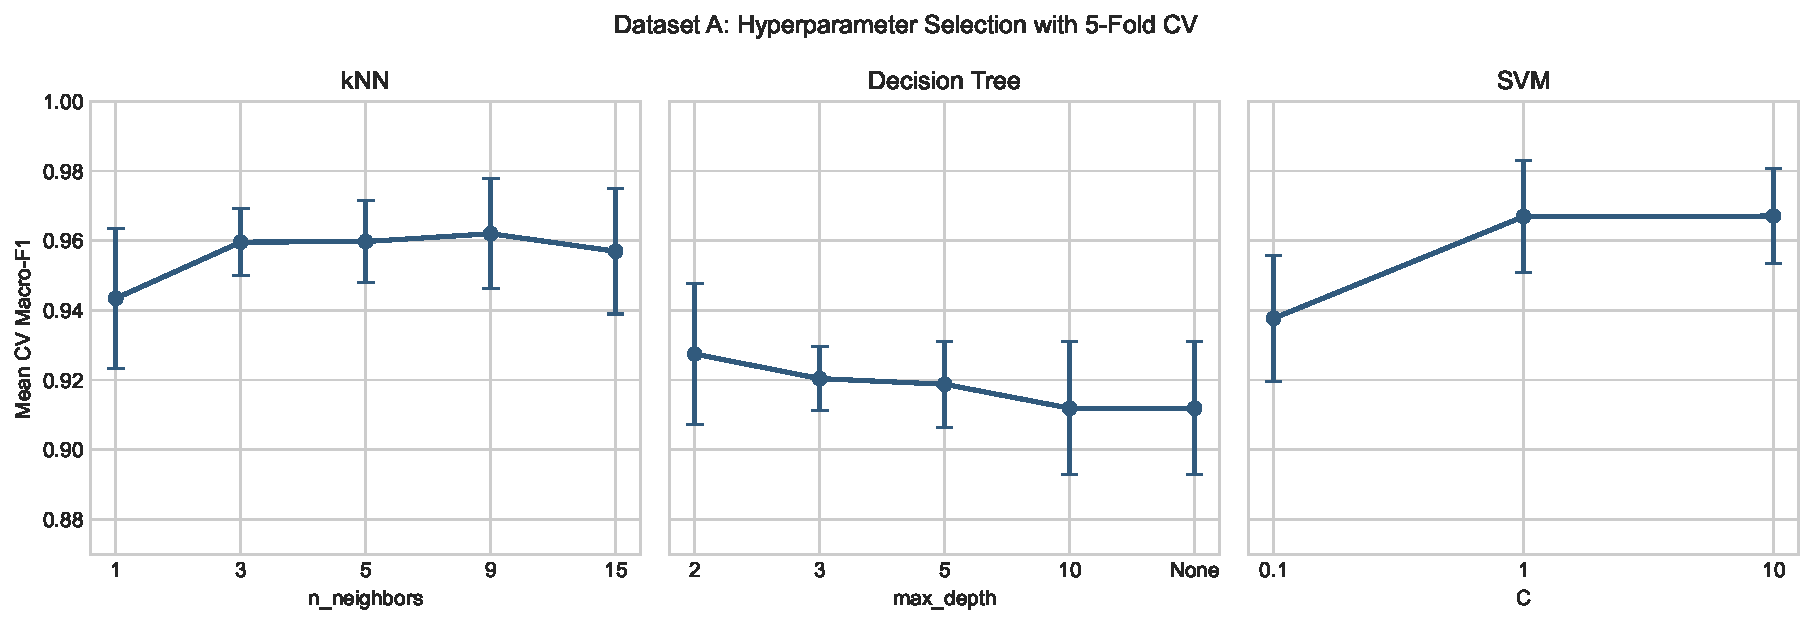
\includegraphics[width=0.92\linewidth]{cv_hyperparameters.pdf}
\par\small Figure 2：候選參數的 training-only CV Macro-F1；error bars 為五折母體標準差。
\end{minipage}
\end{center}

\q{16}{選定設定。}
主要依照平均 Macro-F1 選擇參數，若分數相同，則參考標準差與模型複雜度：kNN 選 $k=9$（.9620$\pm$.0158）、Tree 選 depth 2（.9275$\pm$.0202）、SVM 選 $C=10$（.9671$\pm$.0136）。SVM 的 $C=10$ 與 $C=1$ 平均分數非常接近，但前者的標準差也較小，因此仍選擇 $C=10$。上述選擇均依據交叉驗證結果，未參考測試集分數。

\q{17}{敏感度與「最高 training performance」問題。}
比較各候選設定的平均 Macro-F1，kNN 的最大差距為 0.0186、Decision Tree 為 0.0156、SVM 為 0.0294，因此在本次設定範圍內，SVM 對參數變化最敏感。訓練分數高也不代表泛化效果最好。例如未限制深度的決策樹平均僅 .9119，低於深度 2 的 .9275，顯示模型複雜度增加未必帶來更好的交叉驗證表現。

\q{18}{設定鎖定後的固定 test 一次評估。}
\begin{center}
\compacttable
\begin{tabular}{llrrrrrr}
\toprule
模型 & CV 選定 & Raw Acc. & Raw F1 & Scaled Acc. & Scaled F1 & Final Acc. & Final F1 \\
\midrule
kNN & $k=9$ & .9123 & .9066 & .9561 & .9526 & .9737 & .9713 \\
Tree & $d=2$ & .9123 & .9075 & .9123 & .9075 & .8947 & .8907 \\
SVM & $C=10$ & .9298 & .9230 & .9825 & .9812 & .9737 & .9719 \\
\bottomrule
\end{tabular}
\end{center}
kNN 的提升主要先來自標準化（Macro-F1 +.0460），再經交叉驗證選參提高到 .9713。SVM 在 $C=1$ 且標準化時的測試分數為 .9812，改用交叉驗證選出的 $C=10$ 後則是 .9719；雖然略低，仍不應根據測試結果回頭改選參數。Decision Tree 選擇深度 2 後，測試 Macro-F1 也降至 .8907。這些結果提醒我們：交叉驗證選出的參數不保證在單次測試切分中一定進步。

\section*{Part 5：Dataset B 與跨資料集歸納}
\vspace{-0.5em}

\q{19}{Digits 資料摘要。}
Digits 有 1797 筆、64 個像素特徵與 10 類；各類筆數依 0--9 為 178、182、177、183、181、182、181、179、174、180，固定切分為 1437/360。相較 Dataset A，Digits 樣本較多、類別由 2 增至 10，且特徵是結構化的 $8\times8$ 灰階像素（0--16），而 A 是 30 個量測尺度差異很大的連續醫療特徵。

\q{20}{比較基準。}
Dataset B 不另外進行超參數搜尋，沿用 Part 2 的 baseline 模型設定。依題目要求，kNN 與 SVM 先標準化，其餘模型使用原始特徵；StandardScaler 只在 Dataset B 的訓練集上 fit。所有模型仍使用相同的資料切分。

\q{21}{五模型結果與最佳模型混淆矩陣。}
\begin{center}
\compacttable
\begin{tabular}{cllrr}
\toprule
排名 & 分類器 & 設定 & Accuracy & Macro-F1 \\
\midrule
1 & SVM & Scaled, RBF, $C=1$ & 0.9750 & 0.9748 \\
2 & kNN & Scaled, $k=5$ & 0.9639 & 0.9634 \\
3 & Random Forest & Raw, 200 trees & 0.9639 & 0.9634 \\
4 & Decision Tree & Raw, seed 42 & 0.8222 & 0.8209 \\
5 & Gaussian NB & Raw, defaults & 0.8111 & 0.8137 \\
\bottomrule
\end{tabular}
\end{center}
排名仍先依 Macro-F1、再依 Accuracy。SVM 在 360 筆 test 中正確 351 筆；錯誤主要出現在 8 被判為 1/4，以及 9 被判為 6/7。

\begin{center}
\begin{minipage}{0.72\linewidth}
\centering
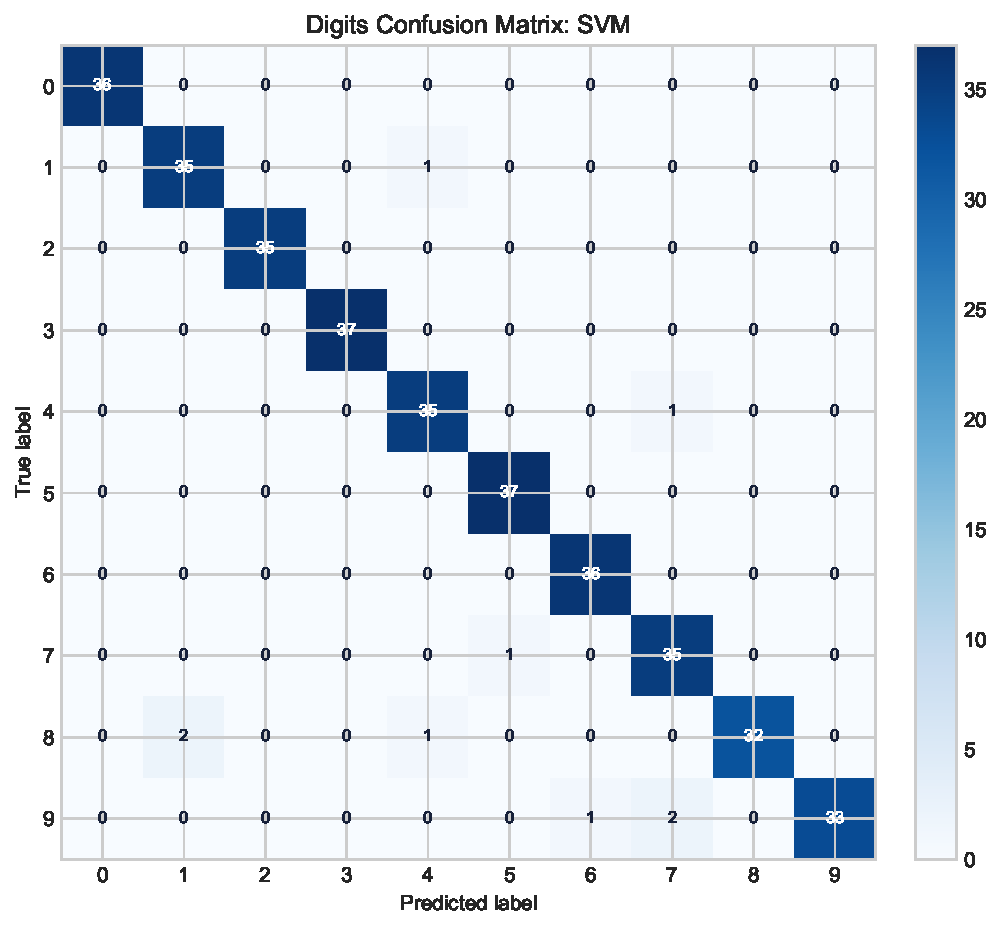
\includegraphics[width=0.67\linewidth]{digits_confusion_matrix.pdf}
\par\small Figure 3：Dataset B 最佳模型 SVM 的混淆矩陣；列為真實類別、欄為預測類別。
\end{minipage}
\end{center}

\q{22}{跨資料集名次。}
Dataset A 的 raw baseline 以 Random Forest 第一、Gaussian NB 第二、SVM 第三；到了 Dataset B，SVM 升至第一，kNN 第二，而 Gaussian NB 降到第五。Digits 的像素特徵與多類別結構，可能更適合 SVM 與 kNN 的判別方式；Gaussian NB 的條件獨立假設則較難描述像素之間的關係。單棵決策樹在這組資料上的表現也明顯較低。需要注意的是，Dataset B 的 kNN、SVM 依題目規定使用了標準化，因此排名差異不能完全歸因於資料集本身。

\textcolor{accent}{\textbf{五分類器特性歸納表。}}
\begin{center}
\scriptsize
\rowcolors{2}{lightrow}{white}
\begin{tabularx}{\linewidth}{lC{1.7cm}Y Y Y}
\toprule
模型 & Scaling 敏感？ & 重要參數/特性 & 本作業優點 & 本作業限制 \\
\midrule
Decision Tree & 否；A 分數不變 & max\_depth；單樹規則可讀 & 可解釋、免 scaling & A final F1 .8907；B 僅 .8209，變異較大 \\
Random Forest & 否；A 分數不變 & n\_estimators；多樹投票 & A raw 第一 .9526；B .9634 & 計算與記憶體高於單樹，整體規則較難讀 \\
kNN & 是；A +.0460 F1 & $k$、距離；延遲式學習 & A final .9713；B .9634 & 預測需保留/搜尋訓練樣本，尺度影響大 \\
Gaussian NB & 本次未 scaling & var\_smoothing；條件獨立高斯 & A raw 第二 .9337；快速簡單 & B 最後 .8137，假設與像素相依性不合 \\
SVM & 是；A +.0582 F1 & $C$、RBF kernel；margin & A final .9719；B 第一 .9748 & scaling/調參重要，決策邊界不易解釋 \\
\bottomrule
\end{tabularx}
\end{center}

\q{23}{是否存在 universally best classifier？（200--300 字）}
\label{q23text}
我認為沒有一種分類器能在所有資料集上都保持最佳表現。乳癌資料的原始特徵中，Random Forest 以 Macro-F1 0.9526 排名第一，但標準化後 SVM 升至 0.9812；Digits 則由 SVM 以 0.9748 居首，Random Forest 為 0.9634，顯示模型表現會受到資料特性與前處理方式影響。SVM 與 kNN 對 scaling 明顯敏感，樹模型則完全不變。Random Forest 需要訓練多棵樹，通常比單棵樹耗費更多資源；單棵樹較容易解釋，但本次分數較低。SVM 表現不錯，決策過程卻比較難直觀說明。kNN 訓練便宜，推論卻須保留並搜尋樣本。此外，類別數、樣本量、特徵尺度與資料結構不同，都可能改變模型的相對優勢。因此，選擇分類器時應參考交叉驗證結果，也要考慮解釋性、運算成本及實際應用需求。

\q{24}{實務推薦。}
Dataset A 我會選擇經交叉驗證選出的 RBF SVM（標準化、$C=10$），其最終 Macro-F1 為 .9719，在三個有進行選參的模型中最高。但醫療資料也重視判斷依據，若需要更容易說明的模型，可以考慮 Random Forest，並搭配特徵重要度分析。Dataset B 則推薦標準化後的 SVM（$C=1$），Accuracy 為 .9750、Macro-F1 為 .9748，360 筆測試資料中僅錯 9 筆。若更重視省去標準化流程，也可以考慮 Macro-F1 為 .9634 的 Random Forest。

\section*{實驗限制與補充說明}
\vspace{-0.5em}

\noindent\textbf{實驗限制。}
本次實驗使用固定的訓練集與測試集切分，並僅針對題目指定的超參數範圍進行比較。因此，實驗結果可能受到資料切分及參數設定影響，尚不足以代表各分類器在所有情況下的表現。

\medskip
\noindent\textbf{程式碼與重現方法。}
本作業使用 Python 與 scikit-learn 進行實驗，完整程式碼及相關檔案可由以下連結取得：

\begin{quote}
\url{https://github.com/potato-yen/data_mining_HW/blob/main/HW5/src/hw5_experiments.py}
\end{quote}

下載專案並安裝所需依賴後，可於專案根目錄執行以下指令，重新產生實驗結果及 Part 1 操作記錄單：

\begin{verbatim}
uv run python src/hw5_experiments.py
uv run python src/build_part1_record.py
\end{verbatim}

實驗採用固定隨機種子（\texttt{random\_state=42}），並使用相同的資料切分與評估流程，以確保結果可重現。

\medskip
\noindent\textbf{Generative AI 使用說明。}
本作業使用 OpenAI Codex 輔助程式實作、實驗流程整理及報告文字編修。實驗數據均由程式實際執行產生，並透過輸出紀錄、圖表與測試結果檢查其一致性。


\end{document}
